\section{РЕЗУЛЬТАТЫ}

\subsection{Графический интерфейс}

\subsection{Решение задач}

\textbf{Примеры решения задач Коши}

Задача Коши задаётся как дифференциальное уравнение n-го порядка и его первые n производных. Здесь показан пример решения нежёсткой
задачи Коши 2-го порядка с использованием явного методы Рунге-Кутты 4-го порядка.

$$
\begin{cases}
	y'' + y - \sin(3x) = 0\\
	y(-2) = -1.701\\
	y'(-2) = -0.022\\
	x \in [-2, 10]
\end{cases}
$$

Аналитическое решение:

$$
y(x) = cos(x) + \dfrac{11}{8}sin(x) - \dfrac{sin(3x)}{8}
$$

\begin{figure}
    \begin{tikzpicture}
\begin{axis}[
	xlabel={$x$},
	ylabel={$y$},
	xmin=-2, xmax=10,
	xtick={-2,0.4,2.8,5.2,7.6,10},
	legend style={at={(1,-0.25)},
                  anchor=north east},
	%legend pos=outer north east,
	ymajorgrids=true,
	grid style=dashed,
]

\addplot[
	color=blue,
	mark=square,
	mark size=0.5pt
]
coordinates {
(-2,-1.701)(-1.8,-1.6623)(-1.6,-1.52744)(-1.4,-1.29315)(-1.2,-0.973584)(-1,-0.598089)(-0.8,-0.204209)(-0.6,0.171682)(-0.4,0.503057)(-0.2,0.778319)(-2.77556e-16,1.00072)(0.2,1.18321)(0.4,1.34039)(0.6,1.48018)(0.8,1.59863)(1,1.67948)(1.2,1.69884)(1.4,1.63335)(1.6,1.46903)(1.8,1.2076)(2,0.86814)(2.2,0.483259)(2.4,0.0911642)(2.6,-0.273863)(2.8,-0.589344)(3,-0.848271)(3.2,-1.05744)(3.4,-1.2312)(3.6,-1.38295)(3.8,-1.51751)(4,-1.62713)(4.2,-1.69265)(4.4,-1.68938)(4.6,-1.59586)(4.8,-1.40221)(5,-1.11531)(5.2,-0.758781)(5.4,-0.367836)(5.6,0.0194978)(5.8,0.37172)(6,0.670717)(6.2,0.913931)(6.4,1.11116)(6.6,1.27737)(6.8,1.42413)(7,1.55279)(7.2,1.65192)(7.4,1.69993)(7.6,1.67215)(7.8,1.54973)(8,1.32734)(8.2,1.017)(8.4,0.646472)(8.6,0.25277)(8.8,-0.127071)(9,-0.464929)(9.2,-0.747253)(9.4,-0.97564)(9.6,-1.16226)(9.8,-1.32196)(10,-1.46386)
};
\addlegendentry{Приближённое решение}

\addplot[
	domain=-2:10,
	color=red,
	samples=100
]{cos(deg(x)) + 11 / 8 * sin(deg(x)) - sin(deg(3 * x)) / 8};
\addlegendentry{Аналитическое решение}

\end{axis}
\end{tikzpicture}
    \caption{Решение задачи №1}
    \label{fig:task1}
\end{figure}

Система дифференциальных уравнений порядка $n$ представлена в виде $n$ дифференциальных уравнений 1-го порядка с начальным условием. В
данном примере демонстрируется решение нежёсткой системы из двух уравнений с использованием вложенного метода Фалберга 2-го порядка.

$$
\begin{cases}
    y' = -12y + 10z^2\\
    z' = y - z - z^2\\
    y(0) = 1\\
    z(0) = 1\\
    x \in [0, 3]
\end{cases}
$$

Аналитическое решение:

$$
y(x) = \exp(-2x)\\
z(x) = \exp(-x)
$$

\begin{figure}
    \begin{tikzpicture}
\begin{axis}[
	xlabel={$x$},
	ylabel={$y$},
	xmin=0, xmax=3,
	xtick={0,0.6,1.2,1.8,2.4,3},
	legend style={at={(1,-0.25)},
                  anchor=north east},
	%legend pos=outer north east,
	ymajorgrids=true,
	grid style=dashed,
]

\addplot[
	color=blue,
	mark=square,
	mark size=0.5pt
]
coordinates {
(0,1)(0.1,0.818736)(0.2,0.670337)(0.3,0.548829)(0.4,0.449331)(0.5,0.367879)(0.6,0.301193)(0.7,0.246607)(0.8,0.201908)(0.9,0.165309)(1,0.135333)(1.1,0.110799)(1.2,0.0907136)(1.3,0.0742782)(1.4,0.0608165)(1.5,0.0497931)(1.6,0.0407673)(1.7,0.0333774)(1.8,0.0273256)(1.9,0.0223728)(2,0.0183174)(2.1,0.014997)(2.2,0.0122786)(2.3,0.0100529)(2.4,0.00822309)(2.5,0.00673079)(2.6,0.00551043)(2.7,0.00451147)(2.8,0.00369362)(2.9,0.00302403)(3,0.00247583)
};
\addlegendentry{Приближённое решение №1}

\addplot[
	color=purple,
	mark=square,
	mark size=0.5pt
]
coordinates {
(0,1)(0.1,0.904837)(0.2,0.818729)(0.3,0.740817)(0.4,0.67032)(0.5,0.606531)(0.6,0.548812)(0.7,0.496584)(0.8,0.449328)(0.9,0.406569)(1,0.36788)(1.1,0.332872)(1.2,0.301195)(1.3,0.272531)(1.4,0.246596)(1.5,0.22313)(1.6,0.201896)(1.7,0.182683)(1.8,0.165299)(1.9,0.149569)(2,0.135335)(2.1,0.122456)(2.2,0.110803)(2.3,0.100259)(2.4,0.0907181)(2.5,0.0820848)(2.6,0.0742729)(2.7,0.0672045)(2.8,0.0608087)(2.9,0.0550217)(3,0.0497853)
};
\addlegendentry{Приближённое решение №2}

\addplot[
	domain=0:3,
	color=red,
	samples=100
]{exp(0 - 2 * x)};
\addlegendentry{Аналитическое решение №1}

\addplot[
	domain=0:3,
	color=red,
	samples=100
]{exp(0 - x)};
\addlegendentry{Аналитическое решение №2}

\end{axis}
\end{tikzpicture}
    \caption{Решение задачи №2}
    \label{fig:task2}
\end{figure}

Отдельного внимания стоит пример решения жёсткой задачи уравнений Ван дер Поля.

$$
\begin{cases}
    y'' - 500(1 - y^2)(y + y') = 0\\
    y(0) = 2\\
    y'(0) = 0\\
    x \in [0, 3]
\end{cases}
$$

\begin{figure}
    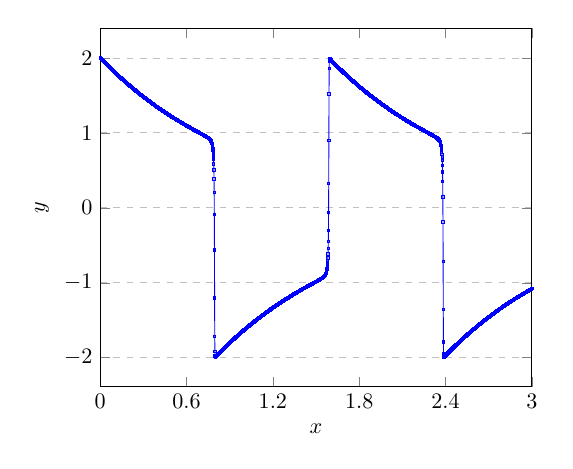
\begin{tikzpicture}[scale = 0.8]
\begin{axis}[
	xlabel={$x$},
	ylabel={$y$},
	xmin=0, xmax=3,
	xtick={0,0.6,1.2,1.8,2.4,3},
	legend style={at={(1,-0.25)},
                  anchor=north east},
	ymajorgrids=true,
	grid style=dashed,
]

\addplot[
	color=blue,
	mark=square,
	mark size=0.5pt
]
coordinates {
(0,2)(0.001,1.99903)(0.002,1.99727)(0.003,1.99532)(0.004,1.99334)(0.005,1.99135)(0.006,1.98936)(0.007,1.98737)(0.008,1.98538)(0.009,1.98339)(0.01,1.98141)(0.011,1.97943)(0.012,1.97745)(0.013,1.97547)(0.014,1.97349)(0.015,1.97152)(0.016,1.96955)(0.017,1.96758)(0.018,1.96561)(0.019,1.96365)(0.02,1.96168)(0.021,1.95972)(0.022,1.95776)(0.023,1.9558)(0.024,1.95384)(0.025,1.95189)(0.026,1.94994)(0.027,1.94799)(0.028,1.94604)(0.029,1.94409)(0.03,1.94215)(0.031,1.94021)(0.032,1.93827)(0.033,1.93633)(0.034,1.93439)(0.035,1.93245)(0.036,1.93052)(0.037,1.92859)(0.038,1.92666)(0.039,1.92473)(0.04,1.92281)(0.041,1.92089)(0.042,1.91896)(0.043,1.91705)(0.044,1.91513)(0.045,1.91321)(0.046,1.9113)(0.047,1.90939)(0.048,1.90748)(0.049,1.90557)(0.05,1.90366)(0.051,1.90176)(0.052,1.89986)(0.053,1.89796)(0.054,1.89606)(0.055,1.89416)(0.056,1.89227)(0.057,1.89037)(0.058,1.88848)(0.059,1.88659)(0.06,1.88471)(0.061,1.88282)(0.062,1.88094)(0.063,1.87906)(0.064,1.87718)(0.065,1.8753)(0.066,1.87342)(0.067,1.87155)(0.068,1.86968)(0.069,1.86781)(0.07,1.86594)(0.071,1.86407)(0.072,1.86221)(0.073,1.86034)(0.074,1.85848)(0.075,1.85662)(0.076,1.85477)(0.077,1.85291)(0.078,1.85106)(0.079,1.84921)(0.08,1.84736)(0.081,1.84551)(0.082,1.84366)(0.083,1.84182)(0.084,1.83998)(0.085,1.83814)(0.086,1.8363)(0.087,1.83446)(0.088,1.83263)(0.089,1.83079)(0.09,1.82896)(0.091,1.82713)(0.092,1.8253)(0.093,1.82348)(0.094,1.82165)(0.095,1.81983)(0.096,1.81801)(0.097,1.81619)(0.098,1.81437)(0.099,1.81256)(0.1,1.81075)(0.101,1.80893)(0.102,1.80713)(0.103,1.80532)(0.104,1.80351)(0.105,1.80171)(0.106,1.7999)(0.107,1.7981)(0.108,1.79631)(0.109,1.79451)(0.11,1.79271)(0.111,1.79092)(0.112,1.78913)(0.113,1.78734)(0.114,1.78555)(0.115,1.78376)(0.116,1.78198)(0.117,1.7802)(0.118,1.77842)(0.119,1.77664)(0.12,1.77486)(0.121,1.77308)(0.122,1.77131)(0.123,1.76954)(0.124,1.76777)(0.125,1.766)(0.126,1.76423)(0.127,1.76247)(0.128,1.7607)(0.129,1.75894)(0.13,1.75718)(0.131,1.75542)(0.132,1.75367)(0.133,1.75191)(0.134,1.75016)(0.135,1.74841)(0.136,1.74666)(0.137,1.74491)(0.138,1.74317)(0.139,1.74142)(0.14,1.73968)(0.141,1.73794)(0.142,1.7362)(0.143,1.73446)(0.144,1.73273)(0.145,1.731)(0.146,1.72926)(0.147,1.72753)(0.148,1.72581)(0.149,1.72408)(0.15,1.72235)(0.151,1.72063)(0.152,1.71891)(0.153,1.71719)(0.154,1.71547)(0.155,1.71375)(0.156,1.71204)(0.157,1.71033)(0.158,1.70862)(0.159,1.70691)(0.16,1.7052)(0.161,1.70349)(0.162,1.70179)(0.163,1.70009)(0.164,1.69838)(0.165,1.69668)(0.166,1.69499)(0.167,1.69329)(0.168,1.6916)(0.169,1.6899)(0.17,1.68821)(0.171,1.68652)(0.172,1.68484)(0.173,1.68315)(0.174,1.68147)(0.175,1.67978)(0.176,1.6781)(0.177,1.67642)(0.178,1.67475)(0.179,1.67307)(0.18,1.6714)(0.181,1.66972)(0.182,1.66805)(0.183,1.66638)(0.184,1.66472)(0.185,1.66305)(0.186,1.66139)(0.187,1.65973)(0.188,1.65806)(0.189,1.65641)(0.19,1.65475)(0.191,1.65309)(0.192,1.65144)(0.193,1.64979)(0.194,1.64813)(0.195,1.64649)(0.196,1.64484)(0.197,1.64319)(0.198,1.64155)(0.199,1.6399)(0.2,1.63826)(0.201,1.63662)(0.202,1.63499)(0.203,1.63335)(0.204,1.63172)(0.205,1.63008)(0.206,1.62845)(0.207,1.62682)(0.208,1.62519)(0.209,1.62357)(0.21,1.62194)(0.211,1.62032)(0.212,1.6187)(0.213,1.61708)(0.214,1.61546)(0.215,1.61384)(0.216,1.61223)(0.217,1.61062)(0.218,1.609)(0.219,1.60739)(0.22,1.60578)(0.221,1.60418)(0.222,1.60257)(0.223,1.60097)(0.224,1.59937)(0.225,1.59777)(0.226,1.59617)(0.227,1.59457)(0.228,1.59297)(0.229,1.59138)(0.23,1.58979)(0.231,1.5882)(0.232,1.58661)(0.233,1.58502)(0.234,1.58343)(0.235,1.58185)(0.236,1.58026)(0.237,1.57868)(0.238,1.5771)(0.239,1.57552)(0.24,1.57395)(0.241,1.57237)(0.242,1.5708)(0.243,1.56923)(0.244,1.56765)(0.245,1.56609)(0.246,1.56452)(0.247,1.56295)(0.248,1.56139)(0.249,1.55983)(0.25,1.55826)(0.251,1.5567)(0.252,1.55515)(0.253,1.55359)(0.254,1.55203)(0.255,1.55048)(0.256,1.54893)(0.257,1.54738)(0.258,1.54583)(0.259,1.54428)(0.26,1.54274)(0.261,1.54119)(0.262,1.53965)(0.263,1.53811)(0.264,1.53657)(0.265,1.53503)(0.266,1.5335)(0.267,1.53196)(0.268,1.53043)(0.269,1.52889)(0.27,1.52736)(0.271,1.52584)(0.272,1.52431)(0.273,1.52278)(0.274,1.52126)(0.275,1.51974)(0.276,1.51821)(0.277,1.51669)(0.278,1.51518)(0.279,1.51366)(0.28,1.51214)(0.281,1.51063)(0.282,1.50912)(0.283,1.50761)(0.284,1.5061)(0.285,1.50459)(0.286,1.50308)(0.287,1.50158)(0.288,1.50008)(0.289,1.49857)(0.29,1.49707)(0.291,1.49558)(0.292,1.49408)(0.293,1.49258)(0.294,1.49109)(0.295,1.4896)(0.296,1.4881)(0.297,1.48661)(0.298,1.48513)(0.299,1.48364)(0.3,1.48215)(0.301,1.48067)(0.302,1.47919)(0.303,1.47771)(0.304,1.47623)(0.305,1.47475)(0.306,1.47327)(0.307,1.4718)(0.308,1.47032)(0.309,1.46885)(0.31,1.46738)(0.311,1.46591)(0.312,1.46444)(0.313,1.46298)(0.314,1.46151)(0.315,1.46005)(0.316,1.45859)(0.317,1.45713)(0.318,1.45567)(0.319,1.45421)(0.32,1.45275)(0.321,1.4513)(0.322,1.44985)(0.323,1.4484)(0.324,1.44694)(0.325,1.4455)(0.326,1.44405)(0.327,1.4426)(0.328,1.44116)(0.329,1.43972)(0.33,1.43827)(0.331,1.43683)(0.332,1.43539)(0.333,1.43396)(0.334,1.43252)(0.335,1.43109)(0.336,1.42965)(0.337,1.42822)(0.338,1.42679)(0.339,1.42536)(0.34,1.42394)(0.341,1.42251)(0.342,1.42108)(0.343,1.41966)(0.344,1.41824)(0.345,1.41682)(0.346,1.4154)(0.347,1.41398)(0.348,1.41257)(0.349,1.41115)(0.35,1.40974)(0.351,1.40833)(0.352,1.40692)(0.353,1.40551)(0.354,1.4041)(0.355,1.40269)(0.356,1.40129)(0.357,1.39989)(0.358,1.39848)(0.359,1.39708)(0.36,1.39568)(0.361,1.39429)(0.362,1.39289)(0.363,1.39149)(0.364,1.3901)(0.365,1.38871)(0.366,1.38732)(0.367,1.38593)(0.368,1.38454)(0.369,1.38315)(0.37,1.38177)(0.371,1.38038)(0.372,1.379)(0.373,1.37762)(0.374,1.37624)(0.375,1.37486)(0.376,1.37348)(0.377,1.37211)(0.378,1.37073)(0.379,1.36936)(0.38,1.36799)(0.381,1.36662)(0.382,1.36525)(0.383,1.36388)(0.384,1.36251)(0.385,1.36115)(0.386,1.35978)(0.387,1.35842)(0.388,1.35706)(0.389,1.3557)(0.39,1.35434)(0.391,1.35299)(0.392,1.35163)(0.393,1.35028)(0.394,1.34892)(0.395,1.34757)(0.396,1.34622)(0.397,1.34487)(0.398,1.34353)(0.399,1.34218)(0.4,1.34083)(0.401,1.33949)(0.402,1.33815)(0.403,1.33681)(0.404,1.33547)(0.405,1.33413)(0.406,1.33279)(0.407,1.33146)(0.408,1.33012)(0.409,1.32879)(0.41,1.32746)(0.411,1.32613)(0.412,1.3248)(0.413,1.32347)(0.414,1.32215)(0.415,1.32082)(0.416,1.3195)(0.417,1.31818)(0.418,1.31685)(0.419,1.31553)(0.42,1.31422)(0.421,1.3129)(0.422,1.31158)(0.423,1.31027)(0.424,1.30896)(0.425,1.30764)(0.426,1.30633)(0.427,1.30502)(0.428,1.30372)(0.429,1.30241)(0.43,1.3011)(0.431,1.2998)(0.432,1.2985)(0.433,1.29719)(0.434,1.29589)(0.435,1.29459)(0.436,1.2933)(0.437,1.292)(0.438,1.29071)(0.439,1.28941)(0.44,1.28812)(0.441,1.28683)(0.442,1.28554)(0.443,1.28425)(0.444,1.28296)(0.445,1.28167)(0.446,1.28039)(0.447,1.27911)(0.448,1.27782)(0.449,1.27654)(0.45,1.27526)(0.451,1.27398)(0.452,1.27271)(0.453,1.27143)(0.454,1.27016)(0.455,1.26888)(0.456,1.26761)(0.457,1.26634)(0.458,1.26507)(0.459,1.2638)(0.46,1.26253)(0.461,1.26127)(0.462,1.26)(0.463,1.25874)(0.464,1.25748)(0.465,1.25621)(0.466,1.25495)(0.467,1.2537)(0.468,1.25244)(0.469,1.25118)(0.47,1.24993)(0.471,1.24867)(0.472,1.24742)(0.473,1.24617)(0.474,1.24492)(0.475,1.24367)(0.476,1.24242)(0.477,1.24118)(0.478,1.23993)(0.479,1.23869)(0.48,1.23745)(0.481,1.2362)(0.482,1.23496)(0.483,1.23373)(0.484,1.23249)(0.485,1.23125)(0.486,1.23002)(0.487,1.22878)(0.488,1.22755)(0.489,1.22632)(0.49,1.22509)(0.491,1.22386)(0.492,1.22263)(0.493,1.2214)(0.494,1.22018)(0.495,1.21895)(0.496,1.21773)(0.497,1.21651)(0.498,1.21529)(0.499,1.21407)(0.5,1.21285)(0.501,1.21163)(0.502,1.21041)(0.503,1.2092)(0.504,1.20799)(0.505,1.20677)(0.506,1.20556)(0.507,1.20435)(0.508,1.20314)(0.509,1.20193)(0.51,1.20073)(0.511,1.19952)(0.512,1.19832)(0.513,1.19711)(0.514,1.19591)(0.515,1.19471)(0.516,1.19351)(0.517,1.19231)(0.518,1.19112)(0.519,1.18992)(0.52,1.18873)(0.521,1.18753)(0.522,1.18634)(0.523,1.18515)(0.524,1.18396)(0.525,1.18277)(0.526,1.18158)(0.527,1.18039)(0.528,1.17921)(0.529,1.17802)(0.53,1.17684)(0.531,1.17566)(0.532,1.17448)(0.533,1.1733)(0.534,1.17212)(0.535,1.17094)(0.536,1.16976)(0.537,1.16859)(0.538,1.16741)(0.539,1.16624)(0.54,1.16507)(0.541,1.1639)(0.542,1.16273)(0.543,1.16156)(0.544,1.16039)(0.545,1.15923)(0.546,1.15806)(0.547,1.1569)(0.548,1.15573)(0.549,1.15457)(0.55,1.15341)(0.551,1.15225)(0.552,1.15109)(0.553,1.14994)(0.554,1.14878)(0.555,1.14762)(0.556,1.14647)(0.557,1.14532)(0.558,1.14417)(0.559,1.14301)(0.56,1.14187)(0.561,1.14072)(0.562,1.13957)(0.563,1.13842)(0.564,1.13728)(0.565,1.13613)(0.566,1.13499)(0.567,1.13385)(0.568,1.13271)(0.569,1.13157)(0.57,1.13043)(0.571,1.12929)(0.572,1.12815)(0.573,1.12702)(0.574,1.12588)(0.575,1.12475)(0.576,1.12362)(0.577,1.12249)(0.578,1.12136)(0.579,1.12023)(0.58,1.1191)(0.581,1.11797)(0.582,1.11685)(0.583,1.11572)(0.584,1.1146)(0.585,1.11348)(0.586,1.11235)(0.587,1.11123)(0.588,1.11011)(0.589,1.109)(0.59,1.10788)(0.591,1.10676)(0.592,1.10565)(0.593,1.10453)(0.594,1.10342)(0.595,1.10231)(0.596,1.10119)(0.597,1.10008)(0.598,1.09898)(0.599,1.09787)(0.6,1.09676)(0.601,1.09565)(0.602,1.09455)(0.603,1.09344)(0.604,1.09234)(0.605,1.09124)(0.606,1.09014)(0.607,1.08904)(0.608,1.08794)(0.609,1.08684)(0.61,1.08574)(0.611,1.08465)(0.612,1.08355)(0.613,1.08246)(0.614,1.08136)(0.615,1.08027)(0.616,1.07918)(0.617,1.07809)(0.618,1.077)(0.619,1.07591)(0.62,1.07482)(0.621,1.07374)(0.622,1.07265)(0.623,1.07157)(0.624,1.07048)(0.625,1.0694)(0.626,1.06832)(0.627,1.06724)(0.628,1.06616)(0.629,1.06508)(0.63,1.064)(0.631,1.06292)(0.632,1.06185)(0.633,1.06077)(0.634,1.0597)(0.635,1.05862)(0.636,1.05755)(0.637,1.05648)(0.638,1.05541)(0.639,1.05434)(0.64,1.05327)(0.641,1.0522)(0.642,1.05113)(0.643,1.05006)(0.644,1.049)(0.645,1.04793)(0.646,1.04687)(0.647,1.0458)(0.648,1.04474)(0.649,1.04368)(0.65,1.04262)(0.651,1.04156)(0.652,1.0405)(0.653,1.03944)(0.654,1.03838)(0.655,1.03733)(0.656,1.03627)(0.657,1.03521)(0.658,1.03416)(0.659,1.0331)(0.66,1.03205)(0.661,1.031)(0.662,1.02994)(0.663,1.02889)(0.664,1.02784)(0.665,1.02679)(0.666,1.02574)(0.667,1.02469)(0.668,1.02364)(0.669,1.0226)(0.67,1.02155)(0.671,1.0205)(0.672,1.01946)(0.673,1.01841)(0.674,1.01737)(0.675,1.01632)(0.676,1.01528)(0.677,1.01423)(0.678,1.01319)(0.679,1.01215)(0.68,1.0111)(0.681,1.01006)(0.682,1.00902)(0.683,1.00798)(0.684,1.00694)(0.685,1.0059)(0.686,1.00486)(0.687,1.00381)(0.688,1.00277)(0.689,1.00173)(0.69,1.00069)(0.691,0.999652)(0.692,0.998612)(0.693,0.997572)(0.694,0.996531)(0.695,0.99549)(0.696,0.994449)(0.697,0.993408)(0.698,0.992367)(0.699,0.991325)(0.7,0.990283)(0.701,0.98924)(0.702,0.988196)(0.703,0.987152)(0.704,0.986107)(0.705,0.985062)(0.706,0.984015)(0.707,0.982968)(0.708,0.981919)(0.709,0.980869)(0.71,0.979818)(0.711,0.978766)(0.712,0.977712)(0.713,0.976656)(0.714,0.975598)(0.715,0.974538)(0.716,0.973477)(0.717,0.972412)(0.718,0.971346)(0.719,0.970276)(0.72,0.969204)(0.721,0.968128)(0.722,0.967049)(0.723,0.965967)(0.724,0.96488)(0.725,0.963789)(0.726,0.962693)(0.727,0.961593)(0.728,0.960487)(0.729,0.959375)(0.73,0.958258)(0.731,0.957133)(0.732,0.956002)(0.733,0.954862)(0.734,0.953715)(0.735,0.952558)(0.736,0.951392)(0.737,0.950215)(0.738,0.949027)(0.739,0.947827)(0.74,0.946614)(0.741,0.945386)(0.742,0.944143)(0.743,0.942884)(0.744,0.941606)(0.745,0.940309)(0.746,0.93899)(0.747,0.937649)(0.748,0.936282)(0.749,0.934888)(0.75,0.933464)(0.751,0.932007)(0.752,0.930515)(0.753,0.928983)(0.754,0.927409)(0.755,0.925788)(0.756,0.924116)(0.757,0.922387)(0.758,0.920596)(0.759,0.918735)(0.76,0.916798)(0.761,0.914776)(0.762,0.912661)(0.763,0.91044)(0.764,0.908102)(0.765,0.905634)(0.766,0.903018)(0.767,0.900236)(0.768,0.897268)(0.769,0.894087)(0.77,0.890665)(0.771,0.886968)(0.772,0.882953)(0.773,0.878574)(0.774,0.873772)(0.775,0.868476)(0.776,0.8626)(0.777,0.85604)(0.778,0.848664)(0.779,0.840307)(0.78,0.830758)(0.781,0.819747)(0.782,0.806916)(0.783,0.791789)(0.784,0.773716)(0.785,0.751788)(0.786,0.724702)(0.787,0.690527)(0.788,0.646295)(0.789,0.587252)(0.79,0.505408)(0.791,0.386616)(0.792,0.204702)(0.793,-0.0885226)(0.794,-0.562711)(0.795,-1.20207)(0.796,-1.71273)(0.797,-1.92098)(0.798,-1.97639)(0.799,-1.98812)(0.8,-1.98931)(0.801,-1.98805)(0.802,-1.98623)(0.803,-1.98428)(0.804,-1.98231)(0.805,-1.98033)(0.806,-1.97835)(0.807,-1.97637)(0.808,-1.97439)(0.809,-1.97242)(0.81,-1.97044)(0.811,-1.96847)(0.812,-1.9665)(0.813,-1.96454)(0.814,-1.96257)(0.815,-1.96061)(0.816,-1.95865)(0.817,-1.95669)(0.818,-1.95473)(0.819,-1.95278)(0.82,-1.95082)(0.821,-1.94887)(0.822,-1.94692)(0.823,-1.94498)(0.824,-1.94303)(0.825,-1.94109)(0.826,-1.93915)(0.827,-1.93721)(0.828,-1.93527)(0.829,-1.93333)(0.83,-1.9314)(0.831,-1.92947)(0.832,-1.92754)(0.833,-1.92561)(0.834,-1.92368)(0.835,-1.92176)(0.836,-1.91984)(0.837,-1.91792)(0.838,-1.916)(0.839,-1.91408)(0.84,-1.91217)(0.841,-1.91025)(0.842,-1.90834)(0.843,-1.90643)(0.844,-1.90453)(0.845,-1.90262)(0.846,-1.90072)(0.847,-1.89882)(0.848,-1.89692)(0.849,-1.89502)(0.85,-1.89313)(0.851,-1.89123)(0.852,-1.88934)(0.853,-1.88745)(0.854,-1.88556)(0.855,-1.88368)(0.856,-1.88179)(0.857,-1.87991)(0.858,-1.87803)(0.859,-1.87615)(0.86,-1.87427)(0.861,-1.8724)(0.862,-1.87053)(0.863,-1.86866)(0.864,-1.86679)(0.865,-1.86492)(0.866,-1.86305)(0.867,-1.86119)(0.868,-1.85933)(0.869,-1.85747)(0.87,-1.85561)(0.871,-1.85375)(0.872,-1.8519)(0.873,-1.85005)(0.874,-1.8482)(0.875,-1.84635)(0.876,-1.8445)(0.877,-1.84266)(0.878,-1.84081)(0.879,-1.83897)(0.88,-1.83713)(0.881,-1.83529)(0.882,-1.83346)(0.883,-1.83162)(0.884,-1.82979)(0.885,-1.82796)(0.886,-1.82613)(0.887,-1.82431)(0.888,-1.82248)(0.889,-1.82066)(0.89,-1.81884)(0.891,-1.81702)(0.892,-1.8152)(0.893,-1.81338)(0.894,-1.81157)(0.895,-1.80976)(0.896,-1.80795)(0.897,-1.80614)(0.898,-1.80433)(0.899,-1.80253)(0.9,-1.80072)(0.901,-1.79892)(0.902,-1.79712)(0.903,-1.79532)(0.904,-1.79353)(0.905,-1.79173)(0.906,-1.78994)(0.907,-1.78815)(0.908,-1.78636)(0.909,-1.78457)(0.91,-1.78279)(0.911,-1.781)(0.912,-1.77922)(0.913,-1.77744)(0.914,-1.77567)(0.915,-1.77389)(0.916,-1.77211)(0.917,-1.77034)(0.918,-1.76857)(0.919,-1.7668)(0.92,-1.76503)(0.921,-1.76327)(0.922,-1.7615)(0.923,-1.75974)(0.924,-1.75798)(0.925,-1.75622)(0.926,-1.75446)(0.927,-1.75271)(0.928,-1.75096)(0.929,-1.7492)(0.93,-1.74745)(0.931,-1.74571)(0.932,-1.74396)(0.933,-1.74221)(0.934,-1.74047)(0.935,-1.73873)(0.936,-1.73699)(0.937,-1.73525)(0.938,-1.73352)(0.939,-1.73178)(0.94,-1.73005)(0.941,-1.72832)(0.942,-1.72659)(0.943,-1.72486)(0.944,-1.72314)(0.945,-1.72141)(0.946,-1.71969)(0.947,-1.71797)(0.948,-1.71625)(0.949,-1.71453)(0.95,-1.71282)(0.951,-1.7111)(0.952,-1.70939)(0.953,-1.70768)(0.954,-1.70597)(0.955,-1.70427)(0.956,-1.70256)(0.957,-1.70086)(0.958,-1.69916)(0.959,-1.69746)(0.96,-1.69576)(0.961,-1.69406)(0.962,-1.69237)(0.963,-1.69067)(0.964,-1.68898)(0.965,-1.68729)(0.966,-1.6856)(0.967,-1.68392)(0.968,-1.68223)(0.969,-1.68055)(0.97,-1.67887)(0.971,-1.67719)(0.972,-1.67551)(0.973,-1.67383)(0.974,-1.67216)(0.975,-1.67048)(0.976,-1.66881)(0.977,-1.66714)(0.978,-1.66547)(0.979,-1.66381)(0.98,-1.66214)(0.981,-1.66048)(0.982,-1.65882)(0.983,-1.65716)(0.984,-1.6555)(0.985,-1.65384)(0.986,-1.65219)(0.987,-1.65053)(0.988,-1.64888)(0.989,-1.64723)(0.99,-1.64558)(0.991,-1.64394)(0.992,-1.64229)(0.993,-1.64065)(0.994,-1.63901)(0.995,-1.63737)(0.996,-1.63573)(0.997,-1.63409)(0.998,-1.63246)(0.999,-1.63082)(1,-1.62919)(1.001,-1.62756)(1.002,-1.62593)(1.003,-1.62431)(1.004,-1.62268)(1.005,-1.62106)(1.006,-1.61943)(1.007,-1.61781)(1.008,-1.61619)(1.009,-1.61458)(1.01,-1.61296)(1.011,-1.61135)(1.012,-1.60973)(1.013,-1.60812)(1.014,-1.60651)(1.015,-1.60491)(1.016,-1.6033)(1.017,-1.6017)(1.018,-1.60009)(1.019,-1.59849)(1.02,-1.59689)(1.021,-1.59529)(1.022,-1.5937)(1.023,-1.5921)(1.024,-1.59051)(1.025,-1.58892)(1.026,-1.58733)(1.027,-1.58574)(1.028,-1.58415)(1.029,-1.58257)(1.03,-1.58098)(1.031,-1.5794)(1.032,-1.57782)(1.033,-1.57624)(1.034,-1.57466)(1.035,-1.57309)(1.036,-1.57151)(1.037,-1.56994)(1.038,-1.56837)(1.039,-1.5668)(1.04,-1.56523)(1.041,-1.56366)(1.042,-1.5621)(1.043,-1.56053)(1.044,-1.55897)(1.045,-1.55741)(1.046,-1.55585)(1.047,-1.5543)(1.048,-1.55274)(1.049,-1.55119)(1.05,-1.54963)(1.051,-1.54808)(1.052,-1.54653)(1.053,-1.54498)(1.054,-1.54344)(1.055,-1.54189)(1.056,-1.54035)(1.057,-1.53881)(1.058,-1.53727)(1.059,-1.53573)(1.06,-1.53419)(1.061,-1.53266)(1.062,-1.53112)(1.063,-1.52959)(1.064,-1.52806)(1.065,-1.52653)(1.066,-1.525)(1.067,-1.52347)(1.068,-1.52195)(1.069,-1.52043)(1.07,-1.5189)(1.071,-1.51738)(1.072,-1.51586)(1.073,-1.51435)(1.074,-1.51283)(1.075,-1.51132)(1.076,-1.5098)(1.077,-1.50829)(1.078,-1.50678)(1.079,-1.50527)(1.08,-1.50377)(1.081,-1.50226)(1.082,-1.50076)(1.083,-1.49926)(1.084,-1.49775)(1.085,-1.49626)(1.086,-1.49476)(1.087,-1.49326)(1.088,-1.49177)(1.089,-1.49027)(1.09,-1.48878)(1.091,-1.48729)(1.092,-1.4858)(1.093,-1.48431)(1.094,-1.48283)(1.095,-1.48134)(1.096,-1.47986)(1.097,-1.47838)(1.098,-1.4769)(1.099,-1.47542)(1.1,-1.47394)(1.101,-1.47247)(1.102,-1.47099)(1.103,-1.46952)(1.104,-1.46805)(1.105,-1.46658)(1.106,-1.46511)(1.107,-1.46364)(1.108,-1.46218)(1.109,-1.46071)(1.11,-1.45925)(1.111,-1.45779)(1.112,-1.45633)(1.113,-1.45487)(1.114,-1.45342)(1.115,-1.45196)(1.116,-1.45051)(1.117,-1.44905)(1.118,-1.4476)(1.119,-1.44615)(1.12,-1.44471)(1.121,-1.44326)(1.122,-1.44181)(1.123,-1.44037)(1.124,-1.43893)(1.125,-1.43749)(1.126,-1.43605)(1.127,-1.43461)(1.128,-1.43317)(1.129,-1.43174)(1.13,-1.4303)(1.131,-1.42887)(1.132,-1.42744)(1.133,-1.42601)(1.134,-1.42458)(1.135,-1.42316)(1.136,-1.42173)(1.137,-1.42031)(1.138,-1.41888)(1.139,-1.41746)(1.14,-1.41604)(1.141,-1.41463)(1.142,-1.41321)(1.143,-1.41179)(1.144,-1.41038)(1.145,-1.40897)(1.146,-1.40756)(1.147,-1.40615)(1.148,-1.40474)(1.149,-1.40333)(1.15,-1.40193)(1.151,-1.40052)(1.152,-1.39912)(1.153,-1.39772)(1.154,-1.39632)(1.155,-1.39492)(1.156,-1.39352)(1.157,-1.39213)(1.158,-1.39073)(1.159,-1.38934)(1.16,-1.38795)(1.161,-1.38656)(1.162,-1.38517)(1.163,-1.38378)(1.164,-1.38239)(1.165,-1.38101)(1.166,-1.37963)(1.167,-1.37824)(1.168,-1.37686)(1.169,-1.37548)(1.17,-1.37411)(1.171,-1.37273)(1.172,-1.37136)(1.173,-1.36998)(1.174,-1.36861)(1.175,-1.36724)(1.176,-1.36587)(1.177,-1.3645)(1.178,-1.36313)(1.179,-1.36177)(1.18,-1.3604)(1.181,-1.35904)(1.182,-1.35768)(1.183,-1.35632)(1.184,-1.35496)(1.185,-1.3536)(1.186,-1.35225)(1.187,-1.35089)(1.188,-1.34954)(1.189,-1.34819)(1.19,-1.34683)(1.191,-1.34549)(1.192,-1.34414)(1.193,-1.34279)(1.194,-1.34144)(1.195,-1.3401)(1.196,-1.33876)(1.197,-1.33742)(1.198,-1.33608)(1.199,-1.33474)(1.2,-1.3334)(1.201,-1.33206)(1.202,-1.33073)(1.203,-1.3294)(1.204,-1.32806)(1.205,-1.32673)(1.206,-1.3254)(1.207,-1.32407)(1.208,-1.32275)(1.209,-1.32142)(1.21,-1.3201)(1.211,-1.31877)(1.212,-1.31745)(1.213,-1.31613)(1.214,-1.31481)(1.215,-1.3135)(1.216,-1.31218)(1.217,-1.31086)(1.218,-1.30955)(1.219,-1.30824)(1.22,-1.30693)(1.221,-1.30562)(1.222,-1.30431)(1.223,-1.303)(1.224,-1.30169)(1.225,-1.30039)(1.226,-1.29909)(1.227,-1.29778)(1.228,-1.29648)(1.229,-1.29518)(1.23,-1.29389)(1.231,-1.29259)(1.232,-1.29129)(1.233,-1.29)(1.234,-1.28871)(1.235,-1.28741)(1.236,-1.28612)(1.237,-1.28483)(1.238,-1.28355)(1.239,-1.28226)(1.24,-1.28097)(1.241,-1.27969)(1.242,-1.27841)(1.243,-1.27712)(1.244,-1.27584)(1.245,-1.27456)(1.246,-1.27329)(1.247,-1.27201)(1.248,-1.27073)(1.249,-1.26946)(1.25,-1.26819)(1.251,-1.26691)(1.252,-1.26564)(1.253,-1.26438)(1.254,-1.26311)(1.255,-1.26184)(1.256,-1.26058)(1.257,-1.25931)(1.258,-1.25805)(1.259,-1.25679)(1.26,-1.25553)(1.261,-1.25427)(1.262,-1.25301)(1.263,-1.25175)(1.264,-1.2505)(1.265,-1.24924)(1.266,-1.24799)(1.267,-1.24674)(1.268,-1.24549)(1.269,-1.24424)(1.27,-1.24299)(1.271,-1.24174)(1.272,-1.2405)(1.273,-1.23925)(1.274,-1.23801)(1.275,-1.23677)(1.276,-1.23553)(1.277,-1.23429)(1.278,-1.23305)(1.279,-1.23181)(1.28,-1.23058)(1.281,-1.22934)(1.282,-1.22811)(1.283,-1.22688)(1.284,-1.22564)(1.285,-1.22441)(1.286,-1.22319)(1.287,-1.22196)(1.288,-1.22073)(1.289,-1.21951)(1.29,-1.21828)(1.291,-1.21706)(1.292,-1.21584)(1.293,-1.21462)(1.294,-1.2134)(1.295,-1.21218)(1.296,-1.21097)(1.297,-1.20975)(1.298,-1.20854)(1.299,-1.20732)(1.3,-1.20611)(1.301,-1.2049)(1.302,-1.20369)(1.303,-1.20248)(1.304,-1.20127)(1.305,-1.20007)(1.306,-1.19886)(1.307,-1.19766)(1.308,-1.19646)(1.309,-1.19526)(1.31,-1.19406)(1.311,-1.19286)(1.312,-1.19166)(1.313,-1.19046)(1.314,-1.18927)(1.315,-1.18807)(1.316,-1.18688)(1.317,-1.18569)(1.318,-1.1845)(1.319,-1.18331)(1.32,-1.18212)(1.321,-1.18093)(1.322,-1.17975)(1.323,-1.17856)(1.324,-1.17738)(1.325,-1.17619)(1.326,-1.17501)(1.327,-1.17383)(1.328,-1.17265)(1.329,-1.17147)(1.33,-1.1703)(1.331,-1.16912)(1.332,-1.16795)(1.333,-1.16677)(1.334,-1.1656)(1.335,-1.16443)(1.336,-1.16326)(1.337,-1.16209)(1.338,-1.16092)(1.339,-1.15975)(1.34,-1.15859)(1.341,-1.15742)(1.342,-1.15626)(1.343,-1.1551)(1.344,-1.15394)(1.345,-1.15278)(1.346,-1.15162)(1.347,-1.15046)(1.348,-1.1493)(1.349,-1.14815)(1.35,-1.14699)(1.351,-1.14584)(1.352,-1.14469)(1.353,-1.14354)(1.354,-1.14239)(1.355,-1.14124)(1.356,-1.14009)(1.357,-1.13894)(1.358,-1.1378)(1.359,-1.13665)(1.36,-1.13551)(1.361,-1.13437)(1.362,-1.13322)(1.363,-1.13208)(1.364,-1.13095)(1.365,-1.12981)(1.366,-1.12867)(1.367,-1.12753)(1.368,-1.1264)(1.369,-1.12527)(1.37,-1.12413)(1.371,-1.123)(1.372,-1.12187)(1.373,-1.12074)(1.374,-1.11961)(1.375,-1.11848)(1.376,-1.11736)(1.377,-1.11623)(1.378,-1.11511)(1.379,-1.11399)(1.38,-1.11286)(1.381,-1.11174)(1.382,-1.11062)(1.383,-1.1095)(1.384,-1.10838)(1.385,-1.10727)(1.386,-1.10615)(1.387,-1.10504)(1.388,-1.10392)(1.389,-1.10281)(1.39,-1.1017)(1.391,-1.10059)(1.392,-1.09948)(1.393,-1.09837)(1.394,-1.09726)(1.395,-1.09615)(1.396,-1.09505)(1.397,-1.09394)(1.398,-1.09284)(1.399,-1.09174)(1.4,-1.09064)(1.401,-1.08954)(1.402,-1.08844)(1.403,-1.08734)(1.404,-1.08624)(1.405,-1.08514)(1.406,-1.08405)(1.407,-1.08295)(1.408,-1.08186)(1.409,-1.08077)(1.41,-1.07967)(1.411,-1.07858)(1.412,-1.07749)(1.413,-1.0764)(1.414,-1.07532)(1.415,-1.07423)(1.416,-1.07314)(1.417,-1.07206)(1.418,-1.07097)(1.419,-1.06989)(1.42,-1.06881)(1.421,-1.06773)(1.422,-1.06665)(1.423,-1.06557)(1.424,-1.06449)(1.425,-1.06341)(1.426,-1.06233)(1.427,-1.06126)(1.428,-1.06018)(1.429,-1.05911)(1.43,-1.05804)(1.431,-1.05696)(1.432,-1.05589)(1.433,-1.05482)(1.434,-1.05375)(1.435,-1.05268)(1.436,-1.05161)(1.437,-1.05055)(1.438,-1.04948)(1.439,-1.04842)(1.44,-1.04735)(1.441,-1.04629)(1.442,-1.04522)(1.443,-1.04416)(1.444,-1.0431)(1.445,-1.04204)(1.446,-1.04098)(1.447,-1.03992)(1.448,-1.03886)(1.449,-1.0378)(1.45,-1.03675)(1.451,-1.03569)(1.452,-1.03464)(1.453,-1.03358)(1.454,-1.03253)(1.455,-1.03147)(1.456,-1.03042)(1.457,-1.02937)(1.458,-1.02832)(1.459,-1.02727)(1.46,-1.02622)(1.461,-1.02517)(1.462,-1.02412)(1.463,-1.02307)(1.464,-1.02202)(1.465,-1.02098)(1.466,-1.01993)(1.467,-1.01889)(1.468,-1.01784)(1.469,-1.01679)(1.47,-1.01575)(1.471,-1.01471)(1.472,-1.01366)(1.473,-1.01262)(1.474,-1.01158)(1.475,-1.01053)(1.476,-1.00949)(1.477,-1.00845)(1.478,-1.00741)(1.479,-1.00637)(1.48,-1.00533)(1.481,-1.00429)(1.482,-1.00325)(1.483,-1.00221)(1.484,-1.00116)(1.485,-1.00012)(1.486,-0.999084)(1.487,-0.998044)(1.488,-0.997003)(1.489,-0.995962)(1.49,-0.994922)(1.491,-0.993881)(1.492,-0.992839)(1.493,-0.991797)(1.494,-0.990755)(1.495,-0.989713)(1.496,-0.98867)(1.497,-0.987626)(1.498,-0.986581)(1.499,-0.985536)(1.5,-0.98449)(1.501,-0.983443)(1.502,-0.982395)(1.503,-0.981346)(1.504,-0.980295)(1.505,-0.979243)(1.506,-0.97819)(1.507,-0.977135)(1.508,-0.976078)(1.509,-0.975019)(1.51,-0.973959)(1.511,-0.972895)(1.512,-0.97183)(1.513,-0.970762)(1.514,-0.969691)(1.515,-0.968617)(1.516,-0.967539)(1.517,-0.966458)(1.518,-0.965373)(1.519,-0.964284)(1.52,-0.963191)(1.521,-0.962093)(1.522,-0.960989)(1.523,-0.95988)(1.524,-0.958766)(1.525,-0.957644)(1.526,-0.956516)(1.527,-0.95538)(1.528,-0.954236)(1.529,-0.953084)(1.53,-0.951922)(1.531,-0.95075)(1.532,-0.949568)(1.533,-0.948373)(1.534,-0.947166)(1.535,-0.945945)(1.536,-0.944709)(1.537,-0.943457)(1.538,-0.942188)(1.539,-0.9409)(1.54,-0.939591)(1.541,-0.93826)(1.542,-0.936905)(1.543,-0.935524)(1.544,-0.934114)(1.545,-0.932672)(1.546,-0.931196)(1.547,-0.929683)(1.548,-0.928129)(1.549,-0.92653)(1.55,-0.924881)(1.551,-0.923179)(1.552,-0.921416)(1.553,-0.919588)(1.554,-0.917687)(1.555,-0.915704)(1.556,-0.913633)(1.557,-0.911461)(1.558,-0.909178)(1.559,-0.906771)(1.56,-0.904224)(1.561,-0.90152)(1.562,-0.898639)(1.563,-0.895558)(1.564,-0.892249)(1.565,-0.888681)(1.566,-0.884816)(1.567,-0.880609)(1.568,-0.876007)(1.569,-0.870944)(1.57,-0.865343)(1.571,-0.859109)(1.572,-0.852121)(1.573,-0.844231)(1.574,-0.835253)(1.575,-0.824943)(1.576,-0.812988)(1.577,-0.798971)(1.578,-0.782329)(1.579,-0.762284)(1.58,-0.737733)(1.581,-0.707066)(1.582,-0.667854)(1.583,-0.616279)(1.584,-0.546068)(1.585,-0.446371)(1.586,-0.297469)(1.587,-0.0625417)(1.588,0.321351)(1.589,0.904236)(1.59,1.51933)(1.591,1.85586)(1.592,1.96031)(1.593,1.98479)(1.594,1.98899)(1.595,1.98843)(1.596,1.98677)(1.597,1.98486)(1.598,1.98289)(1.599,1.98091)(1.6,1.97893)(1.601,1.97695)(1.602,1.97498)(1.603,1.973)(1.604,1.97103)(1.605,1.96906)(1.606,1.96709)(1.607,1.96512)(1.608,1.96315)(1.609,1.96119)(1.61,1.95923)(1.611,1.95727)(1.612,1.95531)(1.613,1.95335)(1.614,1.9514)(1.615,1.94945)(1.616,1.9475)(1.617,1.94555)(1.618,1.94361)(1.619,1.94166)(1.62,1.93972)(1.621,1.93778)(1.622,1.93584)(1.623,1.9339)(1.624,1.93197)(1.625,1.93004)(1.626,1.92811)(1.627,1.92618)(1.628,1.92425)(1.629,1.92233)(1.63,1.9204)(1.631,1.91848)(1.632,1.91656)(1.633,1.91465)(1.634,1.91273)(1.635,1.91082)(1.636,1.90891)(1.637,1.907)(1.638,1.90509)(1.639,1.90319)(1.64,1.90128)(1.641,1.89938)(1.642,1.89748)(1.643,1.89558)(1.644,1.89369)(1.645,1.89179)(1.646,1.8899)(1.647,1.88801)(1.648,1.88612)(1.649,1.88423)(1.65,1.88235)(1.651,1.88047)(1.652,1.87859)(1.653,1.87671)(1.654,1.87483)(1.655,1.87295)(1.656,1.87108)(1.657,1.86921)(1.658,1.86734)(1.659,1.86547)(1.66,1.8636)(1.661,1.86174)(1.662,1.85988)(1.663,1.85802)(1.664,1.85616)(1.665,1.8543)(1.666,1.85245)(1.667,1.85059)(1.668,1.84874)(1.669,1.84689)(1.67,1.84505)(1.671,1.8432)(1.672,1.84136)(1.673,1.83952)(1.674,1.83767)(1.675,1.83584)(1.676,1.834)(1.677,1.83217)(1.678,1.83033)(1.679,1.8285)(1.68,1.82667)(1.681,1.82485)(1.682,1.82302)(1.683,1.8212)(1.684,1.81937)(1.685,1.81755)(1.686,1.81574)(1.687,1.81392)(1.688,1.8121)(1.689,1.81029)(1.69,1.80848)(1.691,1.80667)(1.692,1.80486)(1.693,1.80306)(1.694,1.80126)(1.695,1.79945)(1.696,1.79765)(1.697,1.79585)(1.698,1.79406)(1.699,1.79226)(1.7,1.79047)(1.701,1.78868)(1.702,1.78689)(1.703,1.7851)(1.704,1.78332)(1.705,1.78153)(1.706,1.77975)(1.707,1.77797)(1.708,1.77619)(1.709,1.77441)(1.71,1.77264)(1.711,1.77087)(1.712,1.76909)(1.713,1.76732)(1.714,1.76556)(1.715,1.76379)(1.716,1.76202)(1.717,1.76026)(1.718,1.7585)(1.719,1.75674)(1.72,1.75498)(1.721,1.75323)(1.722,1.75147)(1.723,1.74972)(1.724,1.74797)(1.725,1.74622)(1.726,1.74448)(1.727,1.74273)(1.728,1.74099)(1.729,1.73924)(1.73,1.7375)(1.731,1.73577)(1.732,1.73403)(1.733,1.73229)(1.734,1.73056)(1.735,1.72883)(1.736,1.7271)(1.737,1.72537)(1.738,1.72365)(1.739,1.72192)(1.74,1.7202)(1.741,1.71848)(1.742,1.71676)(1.743,1.71504)(1.744,1.71332)(1.745,1.71161)(1.746,1.7099)(1.747,1.70819)(1.748,1.70648)(1.749,1.70477)(1.75,1.70307)(1.751,1.70136)(1.752,1.69966)(1.753,1.69796)(1.754,1.69626)(1.755,1.69456)(1.756,1.69287)(1.757,1.69117)(1.758,1.68948)(1.759,1.68779)(1.76,1.6861)(1.761,1.68441)(1.762,1.68273)(1.763,1.68105)(1.764,1.67936)(1.765,1.67768)(1.766,1.676)(1.767,1.67433)(1.768,1.67265)(1.769,1.67098)(1.77,1.66931)(1.771,1.66764)(1.772,1.66597)(1.773,1.6643)(1.774,1.66263)(1.775,1.66097)(1.776,1.65931)(1.777,1.65765)(1.778,1.65599)(1.779,1.65433)(1.78,1.65268)(1.781,1.65102)(1.782,1.64937)(1.783,1.64772)(1.784,1.64607)(1.785,1.64443)(1.786,1.64278)(1.787,1.64114)(1.788,1.63949)(1.789,1.63785)(1.79,1.63621)(1.791,1.63458)(1.792,1.63294)(1.793,1.63131)(1.794,1.62967)(1.795,1.62804)(1.796,1.62641)(1.797,1.62479)(1.798,1.62316)(1.799,1.62154)(1.8,1.61991)(1.801,1.61829)(1.802,1.61667)(1.803,1.61506)(1.804,1.61344)(1.805,1.61182)(1.806,1.61021)(1.807,1.6086)(1.808,1.60699)(1.809,1.60538)(1.81,1.60378)(1.811,1.60217)(1.812,1.60057)(1.813,1.59896)(1.814,1.59736)(1.815,1.59577)(1.816,1.59417)(1.817,1.59257)(1.818,1.59098)(1.819,1.58939)(1.82,1.5878)(1.821,1.58621)(1.822,1.58462)(1.823,1.58303)(1.824,1.58145)(1.825,1.57987)(1.826,1.57829)(1.827,1.57671)(1.828,1.57513)(1.829,1.57355)(1.83,1.57198)(1.831,1.5704)(1.832,1.56883)(1.833,1.56726)(1.834,1.56569)(1.835,1.56413)(1.836,1.56256)(1.837,1.561)(1.838,1.55943)(1.839,1.55787)(1.84,1.55631)(1.841,1.55476)(1.842,1.5532)(1.843,1.55165)(1.844,1.55009)(1.845,1.54854)(1.846,1.54699)(1.847,1.54544)(1.848,1.5439)(1.849,1.54235)(1.85,1.54081)(1.851,1.53926)(1.852,1.53772)(1.853,1.53618)(1.854,1.53465)(1.855,1.53311)(1.856,1.53158)(1.857,1.53004)(1.858,1.52851)(1.859,1.52698)(1.86,1.52545)(1.861,1.52393)(1.862,1.5224)(1.863,1.52088)(1.864,1.51935)(1.865,1.51783)(1.866,1.51631)(1.867,1.5148)(1.868,1.51328)(1.869,1.51176)(1.87,1.51025)(1.871,1.50874)(1.872,1.50723)(1.873,1.50572)(1.874,1.50421)(1.875,1.50271)(1.876,1.5012)(1.877,1.4997)(1.878,1.4982)(1.879,1.4967)(1.88,1.4952)(1.881,1.4937)(1.882,1.49221)(1.883,1.49071)(1.884,1.48922)(1.885,1.48773)(1.886,1.48624)(1.887,1.48475)(1.888,1.48327)(1.889,1.48178)(1.89,1.4803)(1.891,1.47882)(1.892,1.47734)(1.893,1.47586)(1.894,1.47438)(1.895,1.4729)(1.896,1.47143)(1.897,1.46995)(1.898,1.46848)(1.899,1.46701)(1.9,1.46554)(1.901,1.46408)(1.902,1.46261)(1.903,1.46115)(1.904,1.45968)(1.905,1.45822)(1.906,1.45676)(1.907,1.4553)(1.908,1.45385)(1.909,1.45239)(1.91,1.45094)(1.911,1.44948)(1.912,1.44803)(1.913,1.44658)(1.914,1.44513)(1.915,1.44369)(1.916,1.44224)(1.917,1.4408)(1.918,1.43935)(1.919,1.43791)(1.92,1.43647)(1.921,1.43503)(1.922,1.4336)(1.923,1.43216)(1.924,1.43073)(1.925,1.42929)(1.926,1.42786)(1.927,1.42643)(1.928,1.425)(1.929,1.42358)(1.93,1.42215)(1.931,1.42073)(1.932,1.41931)(1.933,1.41788)(1.934,1.41646)(1.935,1.41505)(1.936,1.41363)(1.937,1.41221)(1.938,1.4108)(1.939,1.40939)(1.94,1.40797)(1.941,1.40656)(1.942,1.40515)(1.943,1.40375)(1.944,1.40234)(1.945,1.40094)(1.946,1.39953)(1.947,1.39813)(1.948,1.39673)(1.949,1.39533)(1.95,1.39394)(1.951,1.39254)(1.952,1.39114)(1.953,1.38975)(1.954,1.38836)(1.955,1.38697)(1.956,1.38558)(1.957,1.38419)(1.958,1.3828)(1.959,1.38142)(1.96,1.38004)(1.961,1.37865)(1.962,1.37727)(1.963,1.37589)(1.964,1.37451)(1.965,1.37314)(1.966,1.37176)(1.967,1.37039)(1.968,1.36901)(1.969,1.36764)(1.97,1.36627)(1.971,1.3649)(1.972,1.36354)(1.973,1.36217)(1.974,1.36081)(1.975,1.35944)(1.976,1.35808)(1.977,1.35672)(1.978,1.35536)(1.979,1.354)(1.98,1.35265)(1.981,1.35129)(1.982,1.34994)(1.983,1.34859)(1.984,1.34723)(1.985,1.34588)(1.986,1.34454)(1.987,1.34319)(1.988,1.34184)(1.989,1.3405)(1.99,1.33915)(1.991,1.33781)(1.992,1.33647)(1.993,1.33513)(1.994,1.3338)(1.995,1.33246)(1.996,1.33112)(1.997,1.32979)(1.998,1.32846)(1.999,1.32713)(2,1.3258)(2.001,1.32447)(2.002,1.32314)(2.003,1.32181)(2.004,1.32049)(2.005,1.31917)(2.006,1.31784)(2.007,1.31652)(2.008,1.3152)(2.009,1.31389)(2.01,1.31257)(2.011,1.31125)(2.012,1.30994)(2.013,1.30863)(2.014,1.30731)(2.015,1.306)(2.016,1.3047)(2.017,1.30339)(2.018,1.30208)(2.019,1.30078)(2.02,1.29947)(2.021,1.29817)(2.022,1.29687)(2.023,1.29557)(2.024,1.29427)(2.025,1.29297)(2.026,1.29168)(2.027,1.29038)(2.028,1.28909)(2.029,1.2878)(2.03,1.2865)(2.031,1.28521)(2.032,1.28393)(2.033,1.28264)(2.034,1.28135)(2.035,1.28007)(2.036,1.27878)(2.037,1.2775)(2.038,1.27622)(2.039,1.27494)(2.04,1.27366)(2.041,1.27239)(2.042,1.27111)(2.043,1.26984)(2.044,1.26856)(2.045,1.26729)(2.046,1.26602)(2.047,1.26475)(2.048,1.26348)(2.049,1.26222)(2.05,1.26095)(2.051,1.25968)(2.052,1.25842)(2.053,1.25716)(2.054,1.2559)(2.055,1.25464)(2.056,1.25338)(2.057,1.25212)(2.058,1.25087)(2.059,1.24961)(2.06,1.24836)(2.061,1.24711)(2.062,1.24586)(2.063,1.24461)(2.064,1.24336)(2.065,1.24211)(2.066,1.24087)(2.067,1.23962)(2.068,1.23838)(2.069,1.23713)(2.07,1.23589)(2.071,1.23465)(2.072,1.23341)(2.073,1.23218)(2.074,1.23094)(2.075,1.22971)(2.076,1.22847)(2.077,1.22724)(2.078,1.22601)(2.079,1.22478)(2.08,1.22355)(2.081,1.22232)(2.082,1.22109)(2.083,1.21987)(2.084,1.21865)(2.085,1.21742)(2.086,1.2162)(2.087,1.21498)(2.088,1.21376)(2.089,1.21254)(2.09,1.21133)(2.091,1.21011)(2.092,1.20889)(2.093,1.20768)(2.094,1.20647)(2.095,1.20526)(2.096,1.20405)(2.097,1.20284)(2.098,1.20163)(2.099,1.20043)(2.1,1.19922)(2.101,1.19802)(2.102,1.19681)(2.103,1.19561)(2.104,1.19441)(2.105,1.19321)(2.106,1.19201)(2.107,1.19082)(2.108,1.18962)(2.109,1.18843)(2.11,1.18723)(2.111,1.18604)(2.112,1.18485)(2.113,1.18366)(2.114,1.18247)(2.115,1.18128)(2.116,1.1801)(2.117,1.17891)(2.118,1.17773)(2.119,1.17654)(2.12,1.17536)(2.121,1.17418)(2.122,1.173)(2.123,1.17182)(2.124,1.17065)(2.125,1.16947)(2.126,1.16829)(2.127,1.16712)(2.128,1.16595)(2.129,1.16478)(2.13,1.1636)(2.131,1.16244)(2.132,1.16127)(2.133,1.1601)(2.134,1.15893)(2.135,1.15777)(2.136,1.15661)(2.137,1.15544)(2.138,1.15428)(2.139,1.15312)(2.14,1.15196)(2.141,1.1508)(2.142,1.14965)(2.143,1.14849)(2.144,1.14734)(2.145,1.14618)(2.146,1.14503)(2.147,1.14388)(2.148,1.14273)(2.149,1.14158)(2.15,1.14043)(2.151,1.13928)(2.152,1.13814)(2.153,1.13699)(2.154,1.13585)(2.155,1.1347)(2.156,1.13356)(2.157,1.13242)(2.158,1.13128)(2.159,1.13014)(2.16,1.12901)(2.161,1.12787)(2.162,1.12673)(2.163,1.1256)(2.164,1.12447)(2.165,1.12334)(2.166,1.1222)(2.167,1.12107)(2.168,1.11995)(2.169,1.11882)(2.17,1.11769)(2.171,1.11657)(2.172,1.11544)(2.173,1.11432)(2.174,1.11319)(2.175,1.11207)(2.176,1.11095)(2.177,1.10983)(2.178,1.10872)(2.179,1.1076)(2.18,1.10648)(2.181,1.10537)(2.182,1.10425)(2.183,1.10314)(2.184,1.10203)(2.185,1.10092)(2.186,1.09981)(2.187,1.0987)(2.188,1.09759)(2.189,1.09648)(2.19,1.09538)(2.191,1.09427)(2.192,1.09317)(2.193,1.09206)(2.194,1.09096)(2.195,1.08986)(2.196,1.08876)(2.197,1.08766)(2.198,1.08656)(2.199,1.08547)(2.2,1.08437)(2.201,1.08328)(2.202,1.08218)(2.203,1.08109)(2.204,1.08)(2.205,1.07891)(2.206,1.07782)(2.207,1.07673)(2.208,1.07564)(2.209,1.07455)(2.21,1.07346)(2.211,1.07238)(2.212,1.07129)(2.213,1.07021)(2.214,1.06913)(2.215,1.06805)(2.216,1.06697)(2.217,1.06589)(2.218,1.06481)(2.219,1.06373)(2.22,1.06265)(2.221,1.06158)(2.222,1.0605)(2.223,1.05943)(2.224,1.05835)(2.225,1.05728)(2.226,1.05621)(2.227,1.05514)(2.228,1.05407)(2.229,1.053)(2.23,1.05193)(2.231,1.05086)(2.232,1.0498)(2.233,1.04873)(2.234,1.04767)(2.235,1.0466)(2.236,1.04554)(2.237,1.04448)(2.238,1.04341)(2.239,1.04235)(2.24,1.04129)(2.241,1.04023)(2.242,1.03918)(2.243,1.03812)(2.244,1.03706)(2.245,1.036)(2.246,1.03495)(2.247,1.03389)(2.248,1.03284)(2.249,1.03179)(2.25,1.03073)(2.251,1.02968)(2.252,1.02863)(2.253,1.02758)(2.254,1.02653)(2.255,1.02548)(2.256,1.02443)(2.257,1.02338)(2.258,1.02233)(2.259,1.02129)(2.26,1.02024)(2.261,1.01919)(2.262,1.01815)(2.263,1.0171)(2.264,1.01606)(2.265,1.01502)(2.266,1.01397)(2.267,1.01293)(2.268,1.01189)(2.269,1.01084)(2.27,1.0098)(2.271,1.00876)(2.272,1.00772)(2.273,1.00668)(2.274,1.00564)(2.275,1.00459)(2.276,1.00355)(2.277,1.00251)(2.278,1.00147)(2.279,1.00043)(2.28,0.999392)(2.281,0.998351)(2.282,0.997311)(2.283,0.99627)(2.284,0.995229)(2.285,0.994189)(2.286,0.993147)(2.287,0.992106)(2.288,0.991064)(2.289,0.990021)(2.29,0.988978)(2.291,0.987935)(2.292,0.986891)(2.293,0.985846)(2.294,0.9848)(2.295,0.983753)(2.296,0.982705)(2.297,0.981656)(2.298,0.980606)(2.299,0.979555)(2.3,0.978502)(2.301,0.977447)(2.302,0.976391)(2.303,0.975333)(2.304,0.974273)(2.305,0.97321)(2.306,0.972145)(2.307,0.971078)(2.308,0.970008)(2.309,0.968935)(2.31,0.967858)(2.311,0.966778)(2.312,0.965695)(2.313,0.964607)(2.314,0.963515)(2.315,0.962418)(2.316,0.961316)(2.317,0.960209)(2.318,0.959096)(2.319,0.957977)(2.32,0.95685)(2.321,0.955717)(2.322,0.954576)(2.323,0.953426)(2.324,0.952267)(2.325,0.951098)(2.326,0.949919)(2.327,0.948728)(2.328,0.947524)(2.329,0.946308)(2.33,0.945076)(2.331,0.943829)(2.332,0.942566)(2.333,0.941283)(2.334,0.939981)(2.335,0.938657)(2.336,0.937309)(2.337,0.935935)(2.338,0.934534)(2.339,0.933102)(2.34,0.931636)(2.341,0.930135)(2.342,0.928593)(2.343,0.927008)(2.344,0.925374)(2.345,0.923688)(2.346,0.921944)(2.347,0.920136)(2.348,0.918257)(2.349,0.9163)(2.35,0.914255)(2.351,0.912114)(2.352,0.909866)(2.353,0.907497)(2.354,0.904993)(2.355,0.902337)(2.356,0.899511)(2.357,0.896492)(2.358,0.893254)(2.359,0.889766)(2.36,0.885993)(2.361,0.881892)(2.362,0.877413)(2.363,0.872494)(2.364,0.867062)(2.365,0.861026)(2.366,0.854274)(2.367,0.846669)(2.368,0.838035)(2.369,0.828148)(2.37,0.816718)(2.371,0.803363)(2.372,0.787567)(2.373,0.768626)(2.374,0.745548)(2.375,0.716899)(2.376,0.680535)(2.377,0.633132)(2.378,0.569301)(2.379,0.479866)(2.38,0.348377)(2.381,0.144203)(2.382,-0.187762)(2.383,-0.713838)(2.384,-1.35701)(2.385,-1.78971)(2.386,-1.94333)(2.387,-1.98167)(2.388,-1.98919)(2.389,-1.98939)(2.39,-1.98791)(2.391,-1.98604)(2.392,-1.98408)(2.393,-1.9821)(2.394,-1.98012)(2.395,-1.97814)(2.396,-1.97616)(2.397,-1.97419)(2.398,-1.97221)(2.399,-1.97024)(2.4,-1.96827)(2.401,-1.9663)(2.402,-1.96433)(2.403,-1.96237)(2.404,-1.96041)(2.405,-1.95844)(2.406,-1.95649)(2.407,-1.95453)(2.408,-1.95257)(2.409,-1.95062)(2.41,-1.94867)(2.411,-1.94672)(2.412,-1.94477)(2.413,-1.94283)(2.414,-1.94089)(2.415,-1.93894)(2.416,-1.937)(2.417,-1.93507)(2.418,-1.93313)(2.419,-1.9312)(2.42,-1.92927)(2.421,-1.92734)(2.422,-1.92541)(2.423,-1.92348)(2.424,-1.92156)(2.425,-1.91964)(2.426,-1.91772)(2.427,-1.9158)(2.428,-1.91388)(2.429,-1.91197)(2.43,-1.91006)(2.431,-1.90814)(2.432,-1.90624)(2.433,-1.90433)(2.434,-1.90242)(2.435,-1.90052)(2.436,-1.89862)(2.437,-1.89672)(2.438,-1.89482)(2.439,-1.89293)(2.44,-1.89104)(2.441,-1.88914)(2.442,-1.88725)(2.443,-1.88537)(2.444,-1.88348)(2.445,-1.8816)(2.446,-1.87971)(2.447,-1.87783)(2.448,-1.87596)(2.449,-1.87408)(2.45,-1.8722)(2.451,-1.87033)(2.452,-1.86846)(2.453,-1.86659)(2.454,-1.86472)(2.455,-1.86286)(2.456,-1.861)(2.457,-1.85913)(2.458,-1.85727)(2.459,-1.85542)(2.46,-1.85356)(2.461,-1.85171)(2.462,-1.84985)(2.463,-1.848)(2.464,-1.84616)(2.465,-1.84431)(2.466,-1.84246)(2.467,-1.84062)(2.468,-1.83878)(2.469,-1.83694)(2.47,-1.8351)(2.471,-1.83327)(2.472,-1.83143)(2.473,-1.8296)(2.474,-1.82777)(2.475,-1.82594)(2.476,-1.82412)(2.477,-1.82229)(2.478,-1.82047)(2.479,-1.81865)(2.48,-1.81683)(2.481,-1.81501)(2.482,-1.81319)(2.483,-1.81138)(2.484,-1.80957)(2.485,-1.80776)(2.486,-1.80595)(2.487,-1.80414)(2.488,-1.80234)(2.489,-1.80054)(2.49,-1.79873)(2.491,-1.79693)(2.492,-1.79514)(2.493,-1.79334)(2.494,-1.79155)(2.495,-1.78975)(2.496,-1.78796)(2.497,-1.78618)(2.498,-1.78439)(2.499,-1.7826)(2.5,-1.78082)(2.501,-1.77904)(2.502,-1.77726)(2.503,-1.77548)(2.504,-1.7737)(2.505,-1.77193)(2.506,-1.77016)(2.507,-1.76839)(2.508,-1.76662)(2.509,-1.76485)(2.51,-1.76308)(2.511,-1.76132)(2.512,-1.75956)(2.513,-1.7578)(2.514,-1.75604)(2.515,-1.75428)(2.516,-1.75253)(2.517,-1.75077)(2.518,-1.74902)(2.519,-1.74727)(2.52,-1.74552)(2.521,-1.74378)(2.522,-1.74203)(2.523,-1.74029)(2.524,-1.73855)(2.525,-1.73681)(2.526,-1.73507)(2.527,-1.73334)(2.528,-1.7316)(2.529,-1.72987)(2.53,-1.72814)(2.531,-1.72641)(2.532,-1.72468)(2.533,-1.72296)(2.534,-1.72123)(2.535,-1.71951)(2.536,-1.71779)(2.537,-1.71607)(2.538,-1.71435)(2.539,-1.71264)(2.54,-1.71093)(2.541,-1.70921)(2.542,-1.7075)(2.543,-1.7058)(2.544,-1.70409)(2.545,-1.70238)(2.546,-1.70068)(2.547,-1.69898)(2.548,-1.69728)(2.549,-1.69558)(2.55,-1.69388)(2.551,-1.69219)(2.552,-1.6905)(2.553,-1.6888)(2.554,-1.68712)(2.555,-1.68543)(2.556,-1.68374)(2.557,-1.68206)(2.558,-1.68037)(2.559,-1.67869)(2.56,-1.67701)(2.561,-1.67533)(2.562,-1.67366)(2.563,-1.67198)(2.564,-1.67031)(2.565,-1.66864)(2.566,-1.66697)(2.567,-1.6653)(2.568,-1.66363)(2.569,-1.66197)(2.57,-1.66031)(2.571,-1.65865)(2.572,-1.65699)(2.573,-1.65533)(2.574,-1.65367)(2.575,-1.65202)(2.576,-1.65036)(2.577,-1.64871)(2.578,-1.64706)(2.579,-1.64541)(2.58,-1.64377)(2.581,-1.64212)(2.582,-1.64048)(2.583,-1.63884)(2.584,-1.6372)(2.585,-1.63556)(2.586,-1.63392)(2.587,-1.63229)(2.588,-1.63065)(2.589,-1.62902)(2.59,-1.62739)(2.591,-1.62576)(2.592,-1.62414)(2.593,-1.62251)(2.594,-1.62089)(2.595,-1.61927)(2.596,-1.61765)(2.597,-1.61603)(2.598,-1.61441)(2.599,-1.61279)(2.6,-1.61118)(2.601,-1.60957)(2.602,-1.60796)(2.603,-1.60635)(2.604,-1.60474)(2.605,-1.60313)(2.606,-1.60153)(2.607,-1.59993)(2.608,-1.59833)(2.609,-1.59673)(2.61,-1.59513)(2.611,-1.59353)(2.612,-1.59194)(2.613,-1.59034)(2.614,-1.58875)(2.615,-1.58716)(2.616,-1.58557)(2.617,-1.58399)(2.618,-1.5824)(2.619,-1.58082)(2.62,-1.57924)(2.621,-1.57765)(2.622,-1.57608)(2.623,-1.5745)(2.624,-1.57292)(2.625,-1.57135)(2.626,-1.56978)(2.627,-1.5682)(2.628,-1.56663)(2.629,-1.56507)(2.63,-1.5635)(2.631,-1.56194)(2.632,-1.56037)(2.633,-1.55881)(2.634,-1.55725)(2.635,-1.55569)(2.636,-1.55413)(2.637,-1.55258)(2.638,-1.55102)(2.639,-1.54947)(2.64,-1.54792)(2.641,-1.54637)(2.642,-1.54482)(2.643,-1.54328)(2.644,-1.54173)(2.645,-1.54019)(2.646,-1.53865)(2.647,-1.53711)(2.648,-1.53557)(2.649,-1.53403)(2.65,-1.5325)(2.651,-1.53096)(2.652,-1.52943)(2.653,-1.5279)(2.654,-1.52637)(2.655,-1.52484)(2.656,-1.52332)(2.657,-1.52179)(2.658,-1.52027)(2.659,-1.51875)(2.66,-1.51723)(2.661,-1.51571)(2.662,-1.51419)(2.663,-1.51267)(2.664,-1.51116)(2.665,-1.50965)(2.666,-1.50814)(2.667,-1.50663)(2.668,-1.50512)(2.669,-1.50361)(2.67,-1.50211)(2.671,-1.5006)(2.672,-1.4991)(2.673,-1.4976)(2.674,-1.4961)(2.675,-1.4946)(2.676,-1.49311)(2.677,-1.49161)(2.678,-1.49012)(2.679,-1.48863)(2.68,-1.48714)(2.681,-1.48565)(2.682,-1.48416)(2.683,-1.48267)(2.684,-1.48119)(2.685,-1.47971)(2.686,-1.47822)(2.687,-1.47674)(2.688,-1.47527)(2.689,-1.47379)(2.69,-1.47231)(2.691,-1.47084)(2.692,-1.46937)(2.693,-1.4679)(2.694,-1.46643)(2.695,-1.46496)(2.696,-1.46349)(2.697,-1.46203)(2.698,-1.46056)(2.699,-1.4591)(2.7,-1.45764)(2.701,-1.45618)(2.702,-1.45472)(2.703,-1.45326)(2.704,-1.45181)(2.705,-1.45036)(2.706,-1.4489)(2.707,-1.44745)(2.708,-1.446)(2.709,-1.44455)(2.71,-1.44311)(2.711,-1.44166)(2.712,-1.44022)(2.713,-1.43878)(2.714,-1.43734)(2.715,-1.4359)(2.716,-1.43446)(2.717,-1.43302)(2.718,-1.43159)(2.719,-1.43015)(2.72,-1.42872)(2.721,-1.42729)(2.722,-1.42586)(2.723,-1.42443)(2.724,-1.42301)(2.725,-1.42158)(2.726,-1.42016)(2.727,-1.41874)(2.728,-1.41732)(2.729,-1.4159)(2.73,-1.41448)(2.731,-1.41306)(2.732,-1.41165)(2.733,-1.41023)(2.734,-1.40882)(2.735,-1.40741)(2.736,-1.406)(2.737,-1.40459)(2.738,-1.40319)(2.739,-1.40178)(2.74,-1.40038)(2.741,-1.39897)(2.742,-1.39757)(2.743,-1.39617)(2.744,-1.39477)(2.745,-1.39338)(2.746,-1.39198)(2.747,-1.39059)(2.748,-1.38919)(2.749,-1.3878)(2.75,-1.38641)(2.751,-1.38502)(2.752,-1.38364)(2.753,-1.38225)(2.754,-1.38087)(2.755,-1.37948)(2.756,-1.3781)(2.757,-1.37672)(2.758,-1.37534)(2.759,-1.37396)(2.76,-1.37259)(2.761,-1.37121)(2.762,-1.36984)(2.763,-1.36847)(2.764,-1.3671)(2.765,-1.36573)(2.766,-1.36436)(2.767,-1.36299)(2.768,-1.36163)(2.769,-1.36026)(2.77,-1.3589)(2.771,-1.35754)(2.772,-1.35618)(2.773,-1.35482)(2.774,-1.35346)(2.775,-1.35211)(2.776,-1.35075)(2.777,-1.3494)(2.778,-1.34805)(2.779,-1.34669)(2.78,-1.34535)(2.781,-1.344)(2.782,-1.34265)(2.783,-1.34131)(2.784,-1.33996)(2.785,-1.33862)(2.786,-1.33728)(2.787,-1.33594)(2.788,-1.3346)(2.789,-1.33326)(2.79,-1.33193)(2.791,-1.33059)(2.792,-1.32926)(2.793,-1.32793)(2.794,-1.32659)(2.795,-1.32527)(2.796,-1.32394)(2.797,-1.32261)(2.798,-1.32128)(2.799,-1.31996)(2.8,-1.31864)(2.801,-1.31732)(2.802,-1.316)(2.803,-1.31468)(2.804,-1.31336)(2.805,-1.31204)(2.806,-1.31073)(2.807,-1.30941)(2.808,-1.3081)(2.809,-1.30679)(2.81,-1.30548)(2.811,-1.30417)(2.812,-1.30287)(2.813,-1.30156)(2.814,-1.30025)(2.815,-1.29895)(2.816,-1.29765)(2.817,-1.29635)(2.818,-1.29505)(2.819,-1.29375)(2.82,-1.29245)(2.821,-1.29116)(2.822,-1.28986)(2.823,-1.28857)(2.824,-1.28728)(2.825,-1.28599)(2.826,-1.2847)(2.827,-1.28341)(2.828,-1.28212)(2.829,-1.28084)(2.83,-1.27956)(2.831,-1.27827)(2.832,-1.27699)(2.833,-1.27571)(2.834,-1.27443)(2.835,-1.27315)(2.836,-1.27188)(2.837,-1.2706)(2.838,-1.26933)(2.839,-1.26805)(2.84,-1.26678)(2.841,-1.26551)(2.842,-1.26424)(2.843,-1.26298)(2.844,-1.26171)(2.845,-1.26044)(2.846,-1.25918)(2.847,-1.25792)(2.848,-1.25666)(2.849,-1.2554)(2.85,-1.25414)(2.851,-1.25288)(2.852,-1.25162)(2.853,-1.25037)(2.854,-1.24911)(2.855,-1.24786)(2.856,-1.24661)(2.857,-1.24536)(2.858,-1.24411)(2.859,-1.24286)(2.86,-1.24161)(2.861,-1.24037)(2.862,-1.23912)(2.863,-1.23788)(2.864,-1.23664)(2.865,-1.2354)(2.866,-1.23416)(2.867,-1.23292)(2.868,-1.23168)(2.869,-1.23045)(2.87,-1.22921)(2.871,-1.22798)(2.872,-1.22675)(2.873,-1.22552)(2.874,-1.22429)(2.875,-1.22306)(2.876,-1.22183)(2.877,-1.2206)(2.878,-1.21938)(2.879,-1.21816)(2.88,-1.21693)(2.881,-1.21571)(2.882,-1.21449)(2.883,-1.21327)(2.884,-1.21206)(2.885,-1.21084)(2.886,-1.20962)(2.887,-1.20841)(2.888,-1.2072)(2.889,-1.20598)(2.89,-1.20477)(2.891,-1.20356)(2.892,-1.20236)(2.893,-1.20115)(2.894,-1.19994)(2.895,-1.19874)(2.896,-1.19754)(2.897,-1.19633)(2.898,-1.19513)(2.899,-1.19393)(2.9,-1.19273)(2.901,-1.19154)(2.902,-1.19034)(2.903,-1.18914)(2.904,-1.18795)(2.905,-1.18676)(2.906,-1.18556)(2.907,-1.18437)(2.908,-1.18318)(2.909,-1.182)(2.91,-1.18081)(2.911,-1.17962)(2.912,-1.17844)(2.913,-1.17725)(2.914,-1.17607)(2.915,-1.17489)(2.916,-1.17371)(2.917,-1.17253)(2.918,-1.17135)(2.919,-1.17018)(2.92,-1.169)(2.921,-1.16782)(2.922,-1.16665)(2.923,-1.16548)(2.924,-1.16431)(2.925,-1.16314)(2.926,-1.16197)(2.927,-1.1608)(2.928,-1.15963)(2.929,-1.15847)(2.93,-1.1573)(2.931,-1.15614)(2.932,-1.15498)(2.933,-1.15382)(2.934,-1.15266)(2.935,-1.1515)(2.936,-1.15034)(2.937,-1.14918)(2.938,-1.14803)(2.939,-1.14687)(2.94,-1.14572)(2.941,-1.14457)(2.942,-1.14342)(2.943,-1.14227)(2.944,-1.14112)(2.945,-1.13997)(2.946,-1.13882)(2.947,-1.13768)(2.948,-1.13653)(2.949,-1.13539)(2.95,-1.13425)(2.951,-1.13311)(2.952,-1.13197)(2.953,-1.13083)(2.954,-1.12969)(2.955,-1.12855)(2.956,-1.12742)(2.957,-1.12628)(2.958,-1.12515)(2.959,-1.12401)(2.96,-1.12288)(2.961,-1.12175)(2.962,-1.12062)(2.963,-1.11949)(2.964,-1.11837)(2.965,-1.11724)(2.966,-1.11612)(2.967,-1.11499)(2.968,-1.11387)(2.969,-1.11275)(2.97,-1.11163)(2.971,-1.11051)(2.972,-1.10939)(2.973,-1.10827)(2.974,-1.10715)(2.975,-1.10604)(2.976,-1.10492)(2.977,-1.10381)(2.978,-1.10269)(2.979,-1.10158)(2.98,-1.10047)(2.981,-1.09936)(2.982,-1.09825)(2.983,-1.09715)(2.984,-1.09604)(2.985,-1.09493)(2.986,-1.09383)(2.987,-1.09273)(2.988,-1.09162)(2.989,-1.09052)(2.99,-1.08942)(2.991,-1.08832)(2.992,-1.08722)(2.993,-1.08613)(2.994,-1.08503)(2.995,-1.08393)(2.996,-1.08284)(2.997,-1.08175)(2.998,-1.08065)(2.999,-1.07956)(3,-1.07847)
};
%\addlegendentry{Приближённое решение}

\end{axis}
\end{tikzpicture}
    \caption{Решение задачи №3}
    \label{fig:task3}
\end{figure}

Коэффициент жёсткости данной задачи 500 и по графику видно, что жёсткость таких задач заключается в резком скачке градиента функции.
решение было получено благодаря неявному методу Лобатто 6-го порядка с полной таблицей Бутчера.

%таблица сравнения методов (метод, время, шаги, точность)
%методы гаусса, лобатто и прочие неявные (может быть явные если подойдут)
%протестировать многошаговый адамса полунеявный (вес = 0.6)
